\resourceheading{1}{Sensory Access Walk \& Redesign Checklist}{Sensory access and environmental design}{Teachers, families \& school teams}{Module 1 Sensory Walk and Spring 2026 Pine Brook technology placement}

\vspace{-0.5cm}
\toolsection{What This Resource Is}

This is a structured way to examine a classroom from the learner's path. The reviewer follows one routine from entry through instruction, hands-on work, transition, reset, and exit, recording what students must hear, see, touch, filter, remember, and communicate. The Guggenheim sensory-detective approach and the Michigan Developmental Disabilities Institute checklist similarly consider noise, lighting, crowds, routes, predictability, and quiet space \citep{guggenheimSensory,michigan2025sensory}. Rather than waiting for visible distress, the walk treats the environment itself as evidence and asks what can be redesigned before participation narrows.

\toolsection{When and Why to Use It}

Use the walk before opening a classroom, before a noisy or material-heavy lesson, after a schedule or room change, or when participation changes across routines. It is especially useful in technology, robotics, art, science, cafeteria, arrival, dismissal, and other settings where sound, movement, materials, and transitions accumulate. Repeat it at different times; one calm observation cannot represent every condition. Camp documentation reinforced the same principle by treating stepping back and returning as legitimate participation routes rather than as failure to participate \citep{campEvidence2026}.

\toolsection{Ready-to-Use Sensory Walk}

\small
\renewcommand{\arraystretch}{1.10}
\setlength{\tabcolsep}{4pt}
\begin{longtable}{>{\RaggedRight\arraybackslash}p{0.80in} >{\RaggedRight\arraybackslash}p{2.00in} >{\RaggedRight\arraybackslash}p{1.70in} >{\RaggedRight\arraybackslash}p{2.12in}}
\tableheaderfour{Checkpoint}{Notice Without Judging}{Ask the Learner/Family}{Possible Redesign}
\endfirsthead
\tableheaderfour{Checkpoint}{Notice Without Judging}{Ask the Learner/Family}{Possible Redesign}
\endhead
Entry and preview & Competing greetings, crowding, lighting, odors, unclear first step & What helps you enter and know where to begin? & Visual map, calm entry route, consistent materials, greeting choices \\
\rowcolor{SoftGray}
Directions & Length, pace, spoken-language load, visibility of model & Do you want the step shown, written, modeled, or repeated? & One direction at a time, completed example, first/next/last card \\
Hands-on work & Tool noise, device audio, texture, clutter, peer distance & Which tools or materials are comfortable? What is too much? & Stage materials, lower device volume, non-contact route, quieter location \\
\rowcolor{SoftGray}
Communication access & Whether AAC, gestures, writing, or familiar tools remain available & How can you say stop, different, help, space, or more time? & Keep all modes within reach; preteach sensory and repair messages \\
Transition and cleanup & Abrupt stopping, removal of preferred tools, multiple simultaneous demands & What warning and overlap help you change activities? & Visual countdown, overlap period, chosen carry item, modeled first cleanup step \\
\rowcolor{SoftGray}
Reset and return & Whether leaving is punished, hidden, or dependent on adult permission & Where can you reset? How should others know you are ready to return? & Clearly marked low-sensory area, return card, visible re-entry step \\
Exit and review & What the student could access, avoid, communicate, and influence & What should stay, change, or stop next time? & Student/family review, one environmental change, scheduled recheck \\
\end{longtable}
\normalsize

\toolsection{Implementation Sequence}

\begin{enumerate}
  \item Select one real routine and define its beginning and end.
  \item Walk the route while it is in use and record sensory and communication demands.
  \item Ask learners and families what helps, hurts, or varies rather than inferring preference from behavior.
  \item Change one or two high-impact conditions, reduce unnecessary pressure, and keep a route back into participation open.
  \item Observe again and document whether communication, participation, recovery, or choice changes.
\end{enumerate}

\reflectionbox{\textbf{Practice artifact --- Pine Brook IGNITE sensory walk:} Picture choices, visual steps, movement, and hands-on materials supported access, while Chromebook audio, robot movement, table noise, directions, and cleanup accumulated. One learner joined the blocks activity when a familiar laptop could remain nearby. Removing that unnecessary either--or condition changed participation and created a reason to keep investigating what supported access. In Puzzle Plan terms, the changed condition became part of the evidence; EQUITAS asks whether the redesign expands access while preserving choice.}

\begin{center}
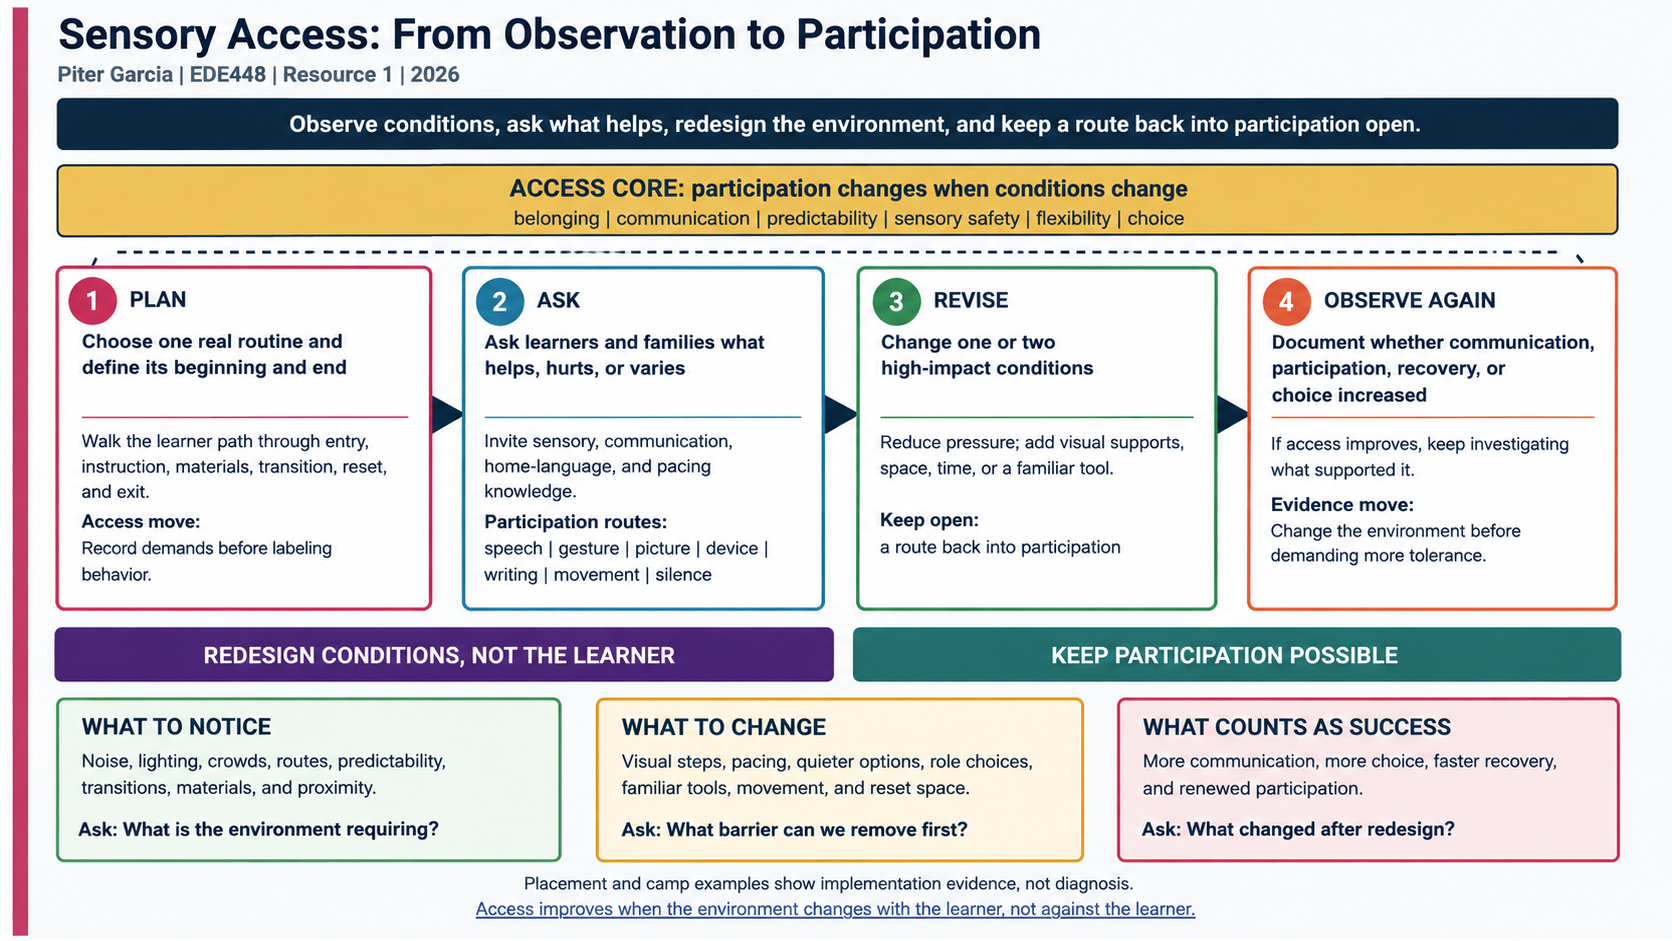
\includegraphics[
  width=1.0\textwidth,
  keepaspectratio
]{assets/artifact-previews/observation_to_participation.png}

\parbox{1.0\textwidth}{\centering\scriptsize
\textbf{\color{DeepNavy}Sensory Access: From Observation to Participation.}
The framework connects observation, learner and family input, environmental redesign, and renewed observation so that changes in communication and participation guide the next instructional decision.}
\end{center}

\adaptationbox{Sensory support is individual and can change across activity, time, fatigue, pain, and experience. The goal is not to make learners tolerate more, but to adjust conditions while protecting communication, participation, and belonging.}

\sourcebox{\scriptsize Guggenheim sensory-environment course resource \citep{guggenheimSensory}; Michigan Developmental Disabilities Institute checklist \citep{michigan2025sensory}.}